\chapter{Introduction}
\label{chp:introduction}

\section{The Problem Description}\label{sec:problem_description}

The original problem description states that the project should be aimed at key management based upon the previous protocol developed for the NUTS project. However, we found major flaws in the underlying protocol, which prevented any further work based on that protocol. We thus focused this project on re-designing the protocol to make sure that NUTS has a trusted transport layer protocol they can build upon. We also shifted the focus away from the NUTS hardware towards a general purpose implementation that would work on all platforms, targeting a setup based on Raspberry Pis communicating over open, unencrypted Wi-Fi. This enables the setup to also be re-used for another course at NTNU, TTM4137 Wireless Network Security, enabling more students to analyze the protocol and try to break it.

The goal of this project is thus to fully describe a new, mutually authenticated protocol, analyze it's security properties, and verify that it works through a sample implementation running on Raspberry Pis.

\section{Results}\label{sec:results}

\begin{figure}[ht!]
\centering
    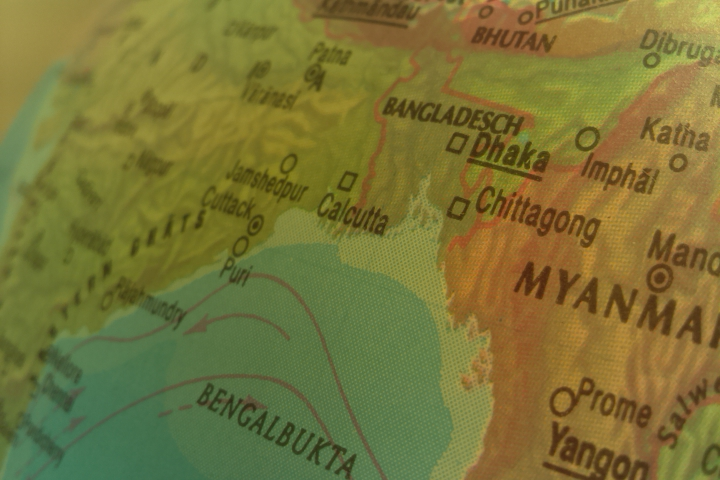
\includegraphics[width=110mm]{orbit-bengal}
    \caption{Image of the Bay of Bengal as taken from the "satellite" in our test environment.}\label{fig:orbit-bengal}
\end{figure}

Two example use cases were developed; one simple "Hello, world" application, and one that could fetch and re-assemble fragmented images from the server. Both of the use cases were tested on the Raspberry Pis in the test environment and completed successfully, using the sample implementation given. The result of the latter, an image from the "satellite" orbiting a globe, can be seen in \autoref{fig:orbit-bengal}. The test environment is documented further in \autoref{chp:experiments}.


\section{Structure of this report}\label{sec:structure}

Before embarking on a description of the protocol, this report will first describe the background for the project and why the protocol is needed, establishing the environment it's intended to operate in. When that's settled, we'll dive into the actual specification of the protocol in \autoref{chp:protocol-description}, taking a step-by-step trip through all the messages exchanged between the parties of a session.

That should bring us to a state where the protocol is well understood. We'll then verify that it adheres to the security properties we intended it to have using a tool called scyther, that's based on formal verification. We'll also briefly discuss how the protocol can be extended and adapted to similar environments.

This brings us into a discussion about random numbers in \autoref{chp:random-numbers}, which is an important prerequisite for the protocol to stay secure. Which again is a natural introduction to failure modes, which we'll discuss in \autoref{chp:failure-modes}. Here we'll look at how the protocol can break, what's necessary to compromise it's integrity, and how it can be mitigated.

That establishes all the theory needed to reason about the protocol, which brings us to the experimental work and the sample implementation. \autoref{chp:experiments} will introduce the API of the sample implementation, and some of the motivation for the choices made. Here we also introduce the test setup and how the protocol have been tested on real hardware.

We then round off in \autoref{chp:conclusions} with some final remarks, and some potential pointers for future work on the protocol.


\section{Terminology}\label{sec:terminology}

Note that \emph{ground station} is used interchangeably with \emph{client} in the rest of this document, and that \emph{satellite} is used interchangeably with \emph{server}. This stems from the project's split focus on both space environments and the test setup. \emph{Packet} and \emph{message} is used somewhat interchangeably for the data unit that is passed between the communicating parties. The symbol $\|$ is used to denote concatenation. MAC-Keccak is a MAC based on Keccak.
